\documentclass[a4paper,12pt]{article}
\usepackage{CJKutf8}
\usepackage{amsthm}
\usepackage{amsmath}
\usepackage{amssymb}
\usepackage{geometry}
\usepackage{subfigure}
\usepackage{tikz}
\usepackage{xcolor}
\usetikzlibrary{patterns}

% 边距
\geometry{left=2.0cm,right=2.0cm,top=2.0cm,bottom=3.0cm}

\newtheorem{theorem}{Theorem}
\newtheorem{lemma}[theorem]{Lemma}
\newtheorem{proposition}[theorem]{Proposition}
\newtheorem{corollary}[theorem]{Corollary}
\newtheorem{exercise}{Exercise}
\newtheorem*{solution}{Solution}
\newtheorem{definition}{Definition}
\theoremstyle{definition}

\makeatletter \renewenvironment{proof}[1][Proof] {\par\pushQED{\qed}\normalfont\topsep6\p@\@plus6\p@\relax\trivlist\item[\hskip\labelsep\bfseries#1\@addpunct{.}]\ignorespaces}{\popQED\endtrivlist\@endpefalse} \makeatother
\makeatletter
\renewenvironment{solution}[1][Solution] {\par\pushQED{\qed}\normalfont\topsep6\p@\@plus6\p@\relax\trivlist\item[\hskip\labelsep\bfseries#1\@addpunct{.}]\ignorespaces}{\popQED\endtrivlist\@endpefalse} \makeatother

% 大题
\newenvironment{problems}{\begin{list}{}{\renewcommand{\makelabel}[1]{\textbf{##1}\hfil}}}{\end{list}}

% 小题
\newenvironment{steps}{\begin{list}{}{\renewcommand{\makelabel}[1]{(##1)\hfil}}}{\end{list}}

% 标题
\title{\small \underline{Mathematical Foundations of Computer Science}\\\Large Project 2}
\author{Log Creative\\\small Student ID: }
\date{\today}

\begin{document}
\maketitle

\noindent\textbf{Warmups}

\begin{problems}
    \item[6] Some of the regions defined by $n$ lines in the plane are infinite, while
    others are bounded. What's the maximum possible number of bounded
    regions?

    \begin{solution}

        First, enumerate the maximum possible number $S_n$ of bounded regions:

        \begin{tabular}{c|c|c|c|c|c|c|c}
            $n$     & 0   & 1 & 2 & 3 & 4 & 5 & $\cdots$ \\
            \hline
            Case    &    & \begin{tikzpicture}
                \draw (-2.2,1.6) -- (-1,2.6);
            \end{tikzpicture}  & 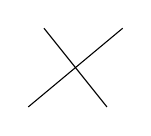
\begin{tikzpicture}
                \draw (-2.2,1.6) -- (-1,2.6);
                \draw (-2,2.6) -- (-1.2,1.6);
                \end{tikzpicture}  & 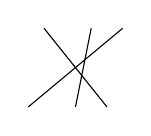
\begin{tikzpicture}
                    \draw (-2.2,1.6) -- (-1,2.6);
                    \draw (-2,2.6) -- (-1.2,1.6);
                    \draw (-1.4,2.6) -- (-1.6,1.6);
                    \end{tikzpicture}  & 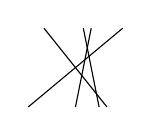
\begin{tikzpicture}
                        \draw (-2.2,1.6) -- (-1,2.6);
                        \draw (-2,2.6) -- (-1.2,1.6);
                        \draw (-1.4,2.6) -- (-1.6,1.6);
                        \draw (-1.5,2.6) -- (-1.3,1.6);
                        \end{tikzpicture}  & 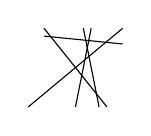
\begin{tikzpicture}
                            \draw (-2.2,1.6) -- (-1,2.6);
                            \draw (-2,2.6) -- (-1.2,1.6);
                            \draw (-1.4,2.6) -- (-1.6,1.6);
                            \draw (-1.5,2.6) -- (-1.3,1.6);
                            \draw (-1,2.4) -- (-2,2.5);
                            \end{tikzpicture}  & $\cdots$\\
            \hline
            $I_n$   & 0  & 0 & 1 & 3 & 6 & 10 & $\cdots$ \\
            \hline
            $\Delta I_n$ &   & 0 & 1 & 2 & 3 & 4 & $\cdots$ \\ 
            \hline
            $S_n$   & 0  & 0 & 0 & 1 & 3 & 6 & $\cdots$ \\
            \hline
            $\Delta S_n$   &   & 0 & 0 & 1 & 2 & 3 & $\cdots$ \\
        \end{tabular}
        
        $I_n$ represents the number of intersections. Three intersections are required to form a bounded region, so no bounded regions while $n\leq 2$. 

        Similar to the observation for finding the maximum possible number $L_n$ of regions, we could know that to get maximum of bounded regions, \textbf{the $n$-th line must hits the previous lines in $n-1$ different places.} Otherwise, there must be a parallel line to the $n$-th line, and the number of bounded regions will reduce, for it doesn't contribute to form the bounded region for the infinite regoin formed by parrell line and the lines it touched, shown in (a).

        \begin{figure}[h]
            \centering
            \subfigure[Bad case with a new parrell line.]{\label{bad}
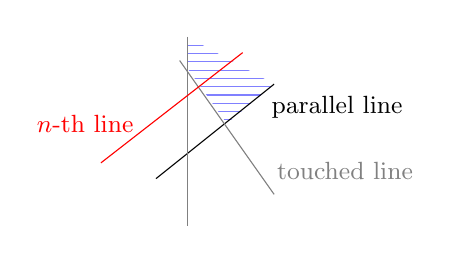
\begin{tikzpicture}
\draw[pattern=horizontal lines,draw=none,pattern color={blue!50}] (-1.9,2.9) -- (-1.9,2.5) -- (-1.4,1.8) -- (-0.8,2.3) -- (-1.9,2.9);
\draw (-2.3,1.1) -- (-0.8,2.3) node (v2) {};
\draw[gray] (-2,2.6) -- (-0.8,0.9);
\draw[gray] (-1.9,2.9) node (v1) {} -- (-1.9,0.5);
\draw[red] (-3,1.3) -- (-1.2,2.7);
\node[red] at (-3.2,1.8) {\small $n$-th line};
\node[gray] at (0.1,1.2) {\small touched line};
\node at (0,2) {\small parallel line};
\end{tikzpicture}}
            \subfigure[Intersections.]{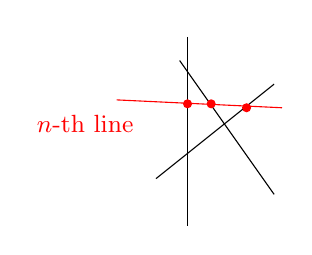
\begin{tikzpicture}
\draw (-2.3,1.1) -- (-0.8,2.3) node (v2) {};
\draw (-2,2.6) -- (-0.8,0.9);
\draw (-1.9,2.9) node (v1) {} -- (-1.9,0.5);
\draw[red] (-2.8,2.1) -- (-0.7,2);
\node[red] at (-3.2,1.8) {\small $n$-th line};
\filldraw[red]  (-1.9,2.05) ellipse (0.05 and 0.05);
\filldraw[red]  (-1.6,2.05) ellipse (0.05 and 0.05);
\filldraw[red]  (-1.15,2) ellipse (0.05 and 0.05);
\end{tikzpicture}}
            \subfigure[Segments split the bounded region and the infinte region.]{
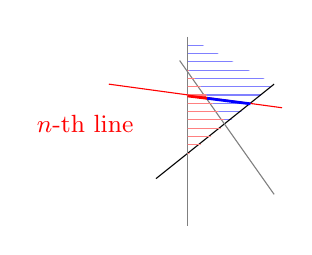
\begin{tikzpicture}
\draw[pattern=horizontal lines,draw=none,pattern color={blue!50}] (-1.9,2.9) -- (-1.9,2.5) node (v3) {} -- (-1.4,1.8) node (v4) {} -- (-0.8,2.3) -- (-1.9,2.9);
\draw (-2.3,1.1) -- (-0.8,2.3) node (v2) {};
\draw[gray] (-2,2.6) -- (-0.8,0.9);
\draw[gray] (-1.9,2.9) node (v1) {} -- (-1.9,0.5);
\draw[red] (-2.9,2.3) -- (-0.7,2);
\node[red] at (-3.2,1.8) {\small $n$-th line};
\draw[pattern=horizontal lines,draw=none,pattern color={red!50}] (-1.9,2.5) -- (-1.9,1.4) -- (-1.4,1.8) -- (-1.9,2.5);
\draw[red,line width=1pt] (-1.9,2.15) -- (-1.65,2.12) node (v5) {};
\draw[blue,line width=1pt] (-1.1,2.05) -- (-1.65,2.12);
\end{tikzpicture}}
        \end{figure}
        
        So, it is the same case for $L_n$ and $S_n$. As the new $n$-th line will add $\Delta I_n=n-1$ intersections, it will only increase $\Delta S_n=(n-1)-1=n-2$ bounded regions \textbf{generated by the middle $(n-1)-1=n-2$ segments}. Because the two end of the new line will not have any intersections to form another bounded regions and point to infinity, shown in (b).

        \textbf{Every Segment introduces $\Delta S_n=1$.} Segements could split bounded regions and infinite regions. When it splits the bounded one (shown in  \textcolor{red}{red}), it will split the region into two because there is no overlapping on intersections, which contributes $\Delta S_n=1$. While it splits (shown in \textcolor{blue}{blue}), it will split th region into a bounded one and an infinite one. Because the two intersections touch two lines seperately and the two lines must intersect and not parallel, then there must introduce a closed triangle or polygon, which also contributes $\Delta S_n=1$. The above is shown in (c).

        Thus, when $n\geq 3$,
        \begin{equation*}
            S_n=\sum_{i=1}^{n-2} i = \frac{(n-2)(n-1)}{2}
        \end{equation*}

        The closed formula is
        \begin{equation*}
            S_n=\left\{
            \begin{aligned}
                &0,&&n=0,1,2;\\
                &\frac{(n-2)(n-1)}{2},&&n\geq 3.
            \end{aligned}
            \right.
        \end{equation*}

    \end{solution}

    \item[7] Let $H(n) = J(n + 1) - J(n)$. Equation (1.8) tells us that $H(2n) = 2$, and
    $H(2n+1) = J(2n+2)-J(2n+1) = (2J(n+1)-1) -  (2J(n)+1)= 2H(n)-2$, for all $n > 1$. Therefore it seems possible to prove that $H(n) = 2$ for all $n$, by induction on $n$. What's wrong here?

    \begin{solution}
        It ignores the case of $n=1$. $H(1)=J(2)-J(1)=1-1=0$, the basic step is wrong for the conclusion of ``$H(n)=2$ for all $n$".

        Now the recurrence is
        \begin{align*}
            H(1)&=0,&&\\
            H(2n)&=2,&&\forall n>1;\\
            H(2n+1)&=2H(n)-2,&&\forall n>1.
        \end{align*}

        As $H(n)=2$ always holds for the even number $n$, it is odd number that needs consideration. List the result of $H(n)$ into a table, where $n$ is an odd number.

        \begin{tabular}[H]{c|c|c|c|c|c|c|c|c|c|c|c}
            $n$ & 1 & 3 & 5 & 7 & 9 & 11 & 13 & 15 & 17 & 19 & $\cdots$ \\
            \hline
            $H(n)$ & 0 & -2 & 2 & -6 & 2 & 2 & 2 & -14 & 2 & 2 & $\cdots$
        \end{tabular}

        And it is discovered that for $n=(\underbrace{1\cdots 1}_{k\text{ of 1's}})_2=\sum_{i=0}^k 1=2^{k+1}-1$, $H(n)\neq 2$. For other odd numbers, $H(n)=2$. And the proof is as follows:

        \begin{description}
            \item[Case 1: $n=2^{k+1}-1(k\in \mathbb{N})$] In this case, the recurrence goes:
            \begin{align*}
                H(2^1-1)&=0&&\\
                H(2^{k+1}-1)&=2H(2^k-1)-2&&k>0
            \end{align*} 
            The last equation could be deduced by:
            \begin{align*}
                H(2^{k+1}-1)-2&=2\left[H(2^k-1)-2\right]\\
                H(2^{k+1}-1)-2&=2^k\cdot (-2)\\
                H(2^{k+1}-1)&=-2^{k+1}+2
            \end{align*}
            \item[Case 2: $n\neq 2^{k+1}-1(k\in \mathbb{N})$] From the closed formula of $J(n)$:
            \begin{align*}
                J(2^m+l)&=2l+1&&\text{for $m\geq 0$ and $0\leq l<2^m$}
            \end{align*} 
            Because $n+1\neq 2^{k+1}$, or $n+1=2^m+l,0<l<2^m$, so $n$ and $n+1$ are in the same domain of $2^m+l$ where $m$ is a specific number. It could be calculate that
            \begin{align*}
                H(n)=J(n+1)-J(n)=2l+1-\left[2(l-1)+1\right] = 2
            \end{align*}
        \end{description}

        To sum up, the closed formula of $H(n)$ is:
        \begin{equation*}
            H(n)=\left\{\begin{aligned}
                &-2^{k+1}+2,&&n=2^{k+1}-1,&&\forall k\in \mathbb{N};\\
                &2,&&\text{otherwise.}
            \end{aligned}\right.
        \end{equation*}
    \end{solution}

\end{problems}

\noindent\textbf{Homework}

\begin{problems}
    \item[8] Solve the recurrence\\
    $Q_0 = \alpha ; Q_1 = \beta ;$\\
    $Q_n = (1 + Q_{n-1})/Q_{n-2} ; \text{ for } n > 1.$\\
    Assume that $Q_n \neq 0 \text{ for all } n \geq 0.$ \emph{Hint:} $Q_4 = (1 + \alpha)/\beta.$

    \begin{solution}
        Due to $Q_n\neq 0$ for all $n\geq 0$, it could be assumed that all the coefficents there are reducible (otherwise a zero on the denominator could introduce a zero on one $Q_n$). And calculate the result based on the recurrence as the following table:

        \begin{tabular}[H]{c|c|c|c|c|c|c|c|c}
            $n$ & 0 & 1 & 2 & 3 & 4 & 5 & 6 & $\cdots$\\
            \hline
            $Q_n$ & $\alpha$ & $\beta$ & $\frac{1+\beta}{\alpha}$ & $\frac{1+\alpha+\beta}{\alpha\beta}$ & $\frac{1+\alpha}{\beta}$ & $\alpha$ & $\beta$ & $\cdots$
        \end{tabular}
        
        And it is discovered that $Q_5=Q_1=\alpha, Q_6=Q_2=\beta$, thus the loop will continue, and the closed formula of the recurrence is:
        \begin{equation*}
            Q_n=\left\{\begin{aligned}
                &\alpha,    &&n \mod 5=0;\\
                &\beta,     &&n \mod 5=1;\\
                &\frac{1+\beta}{\alpha}, && n \mod 5=2;\\
                &\frac{1+\alpha+\beta}{\alpha\beta}, && n \mod 5=3;\\
                &\frac{1+\alpha}{\beta}, &&  n \mod 5=4.
            \end{aligned}\right.
        \end{equation*}
    \end{solution}
    \item[10] Let $Q_n$ be the minimum number of moves needed to transfer a tower of
    $n$ disks from $A$ to $B$ if all moves must be clockwise |that is, from $A$
    to $B$, or from $B$ to the other peg, or from the other peg to $A$. Also let $R_n$
    be the minimum number of moves needed to go from $B$ back to $A$ under
    this restriction. Prove that
    \begin{equation*}
            Q_n=\left\{
                \begin{aligned}
                    &0,&& \text{if } n=0;\\
                    &2R_{n-1}+1,&&\text{if } n>0; 
                \end{aligned}
            \right.
            R_n=\left\{
                \begin{aligned}
                &0,&&\text{if } n=0;\\
                &Q_n+Q_{n-1}+1,&&\text{if } n>0 
            \end{aligned}
                \right.
    \end{equation*}

    (You need not solve these recurrences; we'll see how to do that in Chapter 7.)
    \begin{solution}
        The restriction can be summarized as the left side:

        \begin{center}
            \begin{tikzpicture}[every node/.style={draw,fill=white,minimum size=0.5cm}]
\node (v1) at (-4,1.5) {$A$};
\node (v3) at (-2.5,1.5) {$T$};
\node (v2) at (-1,1.5) {$B$};

\draw[->] (v1) -- (-4,2.5) -- (-1,2.5) -- (v2);
\draw[->]  (v2) edge (v3);
\draw[->]  (v3) edge (v1);
\node[draw=none] at (0.8,2) {$\Rightarrow$};
%\node[draw=none]  (v7) at (3.4,2) {$\circlearrowright$};
%\draw  (v7) ellipse (1.2 and 1.2);
\node (v4) at (2.3,2.5) {$A$};
\node (v5) at (4.5,2.5) {$B$};
\node (v6) at (3.4,0.8) {$T$};

\draw[->]  (v4) edge (v5);
\draw[->]  (v5) edge (v6);
\draw[->]  (v6) edge (v4);
\end{tikzpicture}

        \end{center}
        
        However, the three nodes on the loop, in fact, are \textbf{in the equivalent positions}. Thus, the right side draws them on a equilateral triangle in order to show the equivalence. Thus, any operation follows the clockwise direction is equals $Q$, otherwise equals $R$.

        $Q_0=0$ and $R_0=0$ are obvious.

        Try to solve $Q_n$. As the restriction goes, the minimum number of moves are performed in the following way:
        
        \begin{center}
            \begin{tabular}{cc}
                \begin{tikzpicture}
\tikzstyle{plate}=[draw=gray,text width=2cm,text height=1.5cm, text centered,inner sep=2pt];
\providecommand{\smallbrick}{\begin{tikzpicture}
\node[inner sep=3pt,draw,minimum size=0cm] at (0,0) {$n-1$};
\end{tikzpicture}}
\providecommand{\bigbrick}{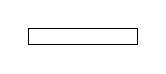
\begin{tikzpicture}
\node[inner sep=3pt,draw,minimum size=0cm] at (0,0) {~~~~~~~~~~~};
\end{tikzpicture}}
\providecommand{\combo}{\begin{tikzpicture}
\node at (0,0) {\smallbrick};
\node at (0,-0.35) {\bigbrick};
\end{tikzpicture}}

\node[plate] (v4) at (1.9,3.9) {\combo};
\node[gray,opacity=0.5] at  (v4) {$A$};
\node[plate] (v5) at (4.9,3.9) {};
\node[gray,opacity=0.5] at (v5) {$B$};
\node[plate] (v6) at (3.4,1.4) {};
\node[gray,opacity=0.5] at (v6) {$T$};

\draw[->,gray]  (v4) edge (v5);
\draw[->,gray]  (v5) edge (v6);
\draw[<-,blue,line width=1pt]  (v6) edge node[right]{$R_{n-1}$} (v4);

\end{tikzpicture}
 &
                \begin{tikzpicture}
\tikzstyle{plate}=[draw=gray,text width=2cm,text height=1.5cm, text centered,inner sep=2pt];
\providecommand{\smallbrick}{\begin{tikzpicture}
\node[inner sep=3pt,draw,minimum size=0cm] at (0,0) {$n-1$};
\end{tikzpicture}}
\providecommand{\bigbrick}{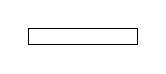
\begin{tikzpicture}
\node[inner sep=3pt,draw,minimum size=0cm] at (0,0) {~~~~~~~~~~~};
\end{tikzpicture}}
\providecommand{\combo}{\begin{tikzpicture}
\node at (0,0) {\smallbrick};
\node at (0,-0.35) {\bigbrick};
\end{tikzpicture}}

\node[plate] (v4) at (1.9,3.9) {\bigbrick};
\node[gray,opacity=0.5] at  (v4) {$A$};
\node[plate] (v5) at (4.9,3.9) {};
\node[gray,opacity=0.5] at (v5) {$B$};
\node[plate] (v6) at (3.4,1.4) {\smallbrick};
\node[gray,opacity=0.5] at (v6) {$T$};

\draw[->,red,line width=1pt]  (v4) edge node[above]{1} (v5);
\draw[->,gray]  (v5) edge (v6);
\draw[->,gray]  (v6) edge (v4);

\end{tikzpicture} \\
                \begin{tikzpicture}
\tikzstyle{plate}=[draw=gray,text width=2cm,text height=1.5cm, text centered,inner sep=2pt];
\providecommand{\smallbrick}{\begin{tikzpicture}
\node[inner sep=3pt,draw,minimum size=0cm] at (0,0) {$n-1$};
\end{tikzpicture}}
\providecommand{\bigbrick}{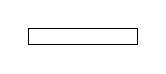
\begin{tikzpicture}
\node[inner sep=3pt,draw,minimum size=0cm] at (0,0) {~~~~~~~~~~~};
\end{tikzpicture}}
\providecommand{\combo}{\begin{tikzpicture}
\node at (0,0) {\smallbrick};
\node at (0,-0.35) {\bigbrick};
\end{tikzpicture}}

\node[plate] (v4) at (1.9,3.9) {};
\node[gray,opacity=0.5] at  (v4) {$A$};
\node[plate] (v5) at (4.9,3.9) {\bigbrick};
\node[gray,opacity=0.5] at (v5) {$B$};
\node[plate] (v6) at (3.4,1.4) {\smallbrick};
\node[gray,opacity=0.5] at (v6) {$T$};

\draw[->,gray]  (v4) edge (v5);
\draw[<-,blue,line width=1pt]  (v5) edge node[left]{$R_{n-1}$} (v6);
\draw[->,gray]  (v6) edge (v4);

\end{tikzpicture}
 &
                \begin{tikzpicture}
\tikzstyle{plate}=[draw=gray,text width=2cm,text height=1.5cm, text centered,inner sep=2pt];
\providecommand{\smallbrick}{\begin{tikzpicture}
\node[inner sep=3pt,draw,minimum size=0cm] at (0,0) {$n-1$};
\end{tikzpicture}}
\providecommand{\bigbrick}{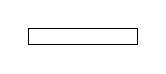
\begin{tikzpicture}
\node[inner sep=3pt,draw,minimum size=0cm] at (0,0) {~~~~~~~~~~~};
\end{tikzpicture}}
\providecommand{\combo}{\begin{tikzpicture}
\node at (0,0) {\smallbrick};
\node at (0,-0.35) {\bigbrick};
\end{tikzpicture}}

\node[plate] (v4) at (1.9,3.9) {};
\node[gray,opacity=0.5] at  (v4) {$A$};
\node[plate] (v5) at (4.9,3.9) {\combo};
\node[gray,opacity=0.5] at (v5) {$B$};
\node[plate] (v6) at (3.4,1.4) {};
\node[gray,opacity=0.5] at (v6) {$T$};

\draw[->,gray]  (v4) edge (v5);
\draw[->,gray]  (v5) edge (v6);
\draw[->,gray]  (v6) edge (v4);

\end{tikzpicture}
            \end{tabular}
        \end{center}
        
        As a result, when $n>0$,
        \begin{equation}\label{eq:q}
            Q_n=R_{n-1}+1+R_{n-1}
        \end{equation}

        So,
        \begin{equation*}
            Q_n=\left\{
                \begin{aligned}
                    &0,&& \text{if } n=0;\\
                    &2R_{n-1}+1,&&\text{if } n>0; 
                \end{aligned}
            \right.
        \end{equation*}

        Then, solve $R_n$. 

        \begin{tikzpicture}
\tikzstyle{plate}=[draw=gray,text width=2cm,text height=1.5cm, text centered,inner sep=2pt];
\providecommand{\smallbrick}{\begin{tikzpicture}
\node[inner sep=3pt,draw,minimum size=0cm] at (0,0) {$n-1$};
\end{tikzpicture}}
\providecommand{\bigbrick}{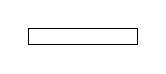
\begin{tikzpicture}
\node[inner sep=3pt,draw,minimum size=0cm] at (0,0) {~~~~~~~~~~~};
\end{tikzpicture}}
\providecommand{\combo}{\begin{tikzpicture}
\node at (0,0) {\smallbrick};
\node at (0,-0.35) {\bigbrick};
\end{tikzpicture}}

\node[plate] (v4) at (1.9,3.9) {};
\node[gray,opacity=0.5] at  (v4) {$A$};
\node[plate] (v5) at (4.9,3.9) {\combo};
\node[gray,opacity=0.5] at (v5) {$B$};
\node[plate] (v6) at (3.4,1.4) {};
\node[gray,opacity=0.5] at (v6) {$T$};

\draw[<-,blue,line width=1pt]  (v4) edge node[below]{$R_{n-1}$} (v5);
\draw[->,gray]  (v5) edge (v6);
\draw[->,gray]  (v6) edge (v4);

\end{tikzpicture}
        \begin{tikzpicture}
\tikzstyle{plate}=[draw=gray,text width=2cm,text height=1.5cm, text centered,inner sep=2pt];
\providecommand{\smallbrick}{\begin{tikzpicture}
\node[inner sep=3pt,draw,minimum size=0cm] at (0,0) {$n-1$};
\end{tikzpicture}}
\providecommand{\bigbrick}{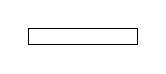
\begin{tikzpicture}
\node[inner sep=3pt,draw,minimum size=0cm] at (0,0) {~~~~~~~~~~~};
\end{tikzpicture}}
\providecommand{\combo}{\begin{tikzpicture}
\node at (0,0) {\smallbrick};
\node at (0,-0.35) {\bigbrick};
\end{tikzpicture}}

\node[plate] (v4) at (1.9,3.9) {\smallbrick};
\node[gray,opacity=0.5] at  (v4) {$A$};
\node[plate] (v5) at (4.9,3.9) {\bigbrick};
\node[gray,opacity=0.5] at (v5) {$B$};
\node[plate] (v6) at (3.4,1.4) {};
\node[gray,opacity=0.5] at (v6) {$T$};

\draw[->,gray]  (v4) edge (v5);
\draw[->,red,line width=1pt]  (v5) edge node[right]{1} (v6);
\draw[->,gray]  (v6) edge (v4);

\end{tikzpicture}
        \begin{tikzpicture}
\tikzstyle{plate}=[draw=gray,text width=2cm,text height=1.5cm, text centered,inner sep=2pt];
\providecommand{\smallbrick}{\begin{tikzpicture}
\node[inner sep=3pt,draw,minimum size=0cm] at (0,0) {$n-1$};
\end{tikzpicture}}
\providecommand{\bigbrick}{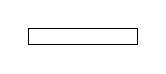
\begin{tikzpicture}
\node[inner sep=3pt,draw,minimum size=0cm] at (0,0) {~~~~~~~~~~~};
\end{tikzpicture}}
\providecommand{\combo}{\begin{tikzpicture}
\node at (0,0) {\smallbrick};
\node at (0,-0.35) {\bigbrick};
\end{tikzpicture}}

\node[plate] (v4) at (1.9,3.9) {\smallbrick};
\node[gray,opacity=0.5] at  (v4) {$A$};
\node[plate] (v5) at (4.9,3.9) {};
\node[gray,opacity=0.5] at (v5) {$B$};
\node[plate] (v6) at (3.4,1.4) {\bigbrick};
\node[gray,opacity=0.5] at (v6) {$T$};

\draw[->,red,line width=1pt]  (v4) edge node[above]{$Q_{n-1}$} (v5);
\draw[->,gray]  (v5) edge (v6);
\draw[->,gray]  (v6) edge (v4);

\end{tikzpicture}
        \begin{tikzpicture}
\tikzstyle{plate}=[draw=gray,text width=2cm,text height=1.5cm, text centered,inner sep=2pt];
\providecommand{\smallbrick}{\begin{tikzpicture}
\node[inner sep=3pt,draw,minimum size=0cm] at (0,0) {$n-1$};
\end{tikzpicture}}
\providecommand{\bigbrick}{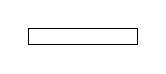
\begin{tikzpicture}
\node[inner sep=3pt,draw,minimum size=0cm] at (0,0) {~~~~~~~~~~~};
\end{tikzpicture}}
\providecommand{\combo}{\begin{tikzpicture}
\node at (0,0) {\smallbrick};
\node at (0,-0.35) {\bigbrick};
\end{tikzpicture}}

\node[plate] (v4) at (1.9,3.9) {};
\node[gray,opacity=0.5] at  (v4) {$A$};
\node[plate] (v5) at (4.9,3.9) {\smallbrick};
\node[gray,opacity=0.5] at (v5) {$B$};
\node[plate] (v6) at (3.4,1.4) {\bigbrick};
\node[gray,opacity=0.5] at (v6) {$T$};

\draw[->,gray]  (v4) edge (v5);
\draw[->,gray]  (v5) edge (v6);
\draw[->,red,line width=1pt]  (v6) edge node[left]{1} (v4);

\end{tikzpicture}

        \begin{tikzpicture}
\tikzstyle{plate}=[draw=gray,text width=2cm,text height=1.5cm, text centered,inner sep=2pt];
\providecommand{\smallbrick}{\begin{tikzpicture}
\node[inner sep=3pt,draw,minimum size=0cm] at (0,0) {$n-1$};
\end{tikzpicture}}
\providecommand{\bigbrick}{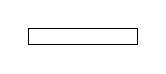
\begin{tikzpicture}
\node[inner sep=3pt,draw,minimum size=0cm] at (0,0) {~~~~~~~~~~~};
\end{tikzpicture}}
\providecommand{\combo}{\begin{tikzpicture}
\node at (0,0) {\smallbrick};
\node at (0,-0.35) {\bigbrick};
\end{tikzpicture}}

\node[plate] (v4) at (1.9,3.9) {\bigbrick};
\node[gray,opacity=0.5] at  (v4) {$A$};
\node[plate] (v5) at (4.9,3.9) {\smallbrick};
\node[gray,opacity=0.5] at (v5) {$B$};
\node[plate] (v6) at (3.4,1.4) {};
\node[gray,opacity=0.5] at (v6) {$T$};

\draw[<-,blue,line width=1pt]  (v4) edge node[below]{$R_{n-1}$} (v5);
\draw[->,gray]  (v5) edge (v6);
\draw[->,gray]  (v6) edge (v4);

\end{tikzpicture}
        \begin{tikzpicture}
\tikzstyle{plate}=[draw=gray,text width=2cm,text height=1.5cm, text centered,inner sep=2pt];
\providecommand{\smallbrick}{\begin{tikzpicture}
\node[inner sep=3pt,draw,minimum size=0cm] at (0,0) {$n-1$};
\end{tikzpicture}}
\providecommand{\bigbrick}{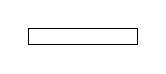
\begin{tikzpicture}
\node[inner sep=3pt,draw,minimum size=0cm] at (0,0) {~~~~~~~~~~~};
\end{tikzpicture}}
\providecommand{\combo}{\begin{tikzpicture}
\node at (0,0) {\smallbrick};
\node at (0,-0.35) {\bigbrick};
\end{tikzpicture}}

\node[plate] (v4) at (1.9,3.9) {\combo};
\node[gray,opacity=0.5] at  (v4) {$A$};
\node[plate] (v5) at (4.9,3.9) {};
\node[gray,opacity=0.5] at (v5) {$B$};
\node[plate] (v6) at (3.4,1.4) {};
\node[gray,opacity=0.5] at (v6) {$T$};

\draw[->,gray]  (v4) edge (v5);
\draw[->,gray]  (v5) edge (v6);
\draw[->,gray]  (v6) edge (v4);

\end{tikzpicture}


        As a result, when $n>0$,
        \begin{equation*}
            R_n=R_{n-1}+1+Q_{n-1}+1+R_{n-1}=Q_{n-1}+2R_{n-1}+1
        \end{equation*}

        Combine Equation \eqref{eq:q}, we could get that
        \begin{equation*}
            R_n=\left\{
                \begin{aligned}
                &0,&&\text{if } n=0;\\
                &Q_n+Q_{n-1}+1,&&\text{if } n>0. 
            \end{aligned}
                \right.
        \end{equation*}

    \end{solution}

\end{problems}

\end{document}
